\documentclass[1p]{elsarticle_modified}
%\bibliographystyle{elsarticle-num}

%\usepackage[colorlinks]{hyperref}
%\usepackage{abbrmath_seonhwa} %\Abb, \Ascr, \Acal ,\Abf, \Afrak
\usepackage{amsfonts}
\usepackage{amssymb}
\usepackage{amsmath}
\usepackage{amsthm}
\usepackage{scalefnt}
\usepackage{amsbsy}
\usepackage{kotex}
\usepackage{caption}
\usepackage{subfig}
\usepackage{color}
\usepackage{graphicx}
\usepackage{xcolor} %% white, black, red, green, blue, cyan, magenta, yellow
\usepackage{float}
\usepackage{setspace}
\usepackage{hyperref}

\usepackage{tikz}
\usetikzlibrary{arrows}

\usepackage{multirow}
\usepackage{array} % fixed length table
\usepackage{hhline}

%%%%%%%%%%%%%%%%%%%%%
\makeatletter
\renewcommand*\env@matrix[1][\arraystretch]{%
	\edef\arraystretch{#1}%
	\hskip -\arraycolsep
	\let\@ifnextchar\new@ifnextchar
	\array{*\c@MaxMatrixCols c}}
\makeatother %https://tex.stackexchange.com/questions/14071/how-can-i-increase-the-line-spacing-in-a-matrix
%%%%%%%%%%%%%%%

\usepackage[normalem]{ulem}

\newcommand{\msout}[1]{\ifmmode\text{\sout{\ensuremath{#1}}}\else\sout{#1}\fi}
%SOURCE: \msout is \stkout macro in https://tex.stackexchange.com/questions/20609/strikeout-in-math-mode

\newcommand{\cancel}[1]{
	\ifmmode
	{\color{red}\msout{#1}}
	\else
	{\color{red}\sout{#1}}
	\fi
}

\newcommand{\add}[1]{
	{\color{blue}\uwave{#1}}
}

\newcommand{\replace}[2]{
	\ifmmode
	{\color{red}\msout{#1}}{\color{blue}\uwave{#2}}
	\else
	{\color{red}\sout{#1}}{\color{blue}\uwave{#2}}
	\fi
}

\newcommand{\Sol}{\mathcal{S}} %segment
\newcommand{\D}{D} %diagram
\newcommand{\A}{\mathcal{A}} %arc


%%%%%%%%%%%%%%%%%%%%%%%%%%%%%5 test

\def\sl{\operatorname{\textup{SL}}(2,\Cbb)}
\def\psl{\operatorname{\textup{PSL}}(2,\Cbb)}
\def\quan{\mkern 1mu \triangleright \mkern 1mu}

\theoremstyle{definition}
\newtheorem{thm}{Theorem}[section]
\newtheorem{prop}[thm]{Proposition}
\newtheorem{lem}[thm]{Lemma}
\newtheorem{ques}[thm]{Question}
\newtheorem{cor}[thm]{Corollary}
\newtheorem{defn}[thm]{Definition}
\newtheorem{exam}[thm]{Example}
\newtheorem{rmk}[thm]{Remark}
\newtheorem{alg}[thm]{Algorithm}

\newcommand{\I}{\sqrt{-1}}
\begin{document}

%\begin{frontmatter}
%
%\title{Boundary parabolic representations of knots up to 8 crossings}
%
%%% Group authors per affiliation:
%\author{Yunhi Cho} 
%\address{Department of Mathematics, University of Seoul, Seoul, Korea}
%\ead{yhcho@uos.ac.kr}
%
%
%\author{Seonhwa Kim} %\fnref{s_kim}}
%\address{Center for Geometry and Physics, Institute for Basic Science, Pohang, 37673, Korea}
%\ead{ryeona17@ibs.re.kr}
%
%\author{Hyuk Kim}
%\address{Department of Mathematical Sciences, Seoul National University, Seoul 08826, Korea}
%\ead{hyukkim@snu.ac.kr}
%
%\author{Seokbeom Yoon}
%\address{Department of Mathematical Sciences, Seoul National University, Seoul, 08826,  Korea}
%\ead{sbyoon15@snu.ac.kr}
%
%\begin{abstract}
%We find all boundary parabolic representation of knots up to 8 crossings.
%
%\end{abstract}
%\begin{keyword}
%    \MSC[2010] 57M25 
%\end{keyword}
%
%\end{frontmatter}

%\linenumbers
%\tableofcontents
%
\newcommand\colored[1]{\textcolor{white}{\rule[-0.35ex]{0.8em}{1.4ex}}\kern-0.8em\color{red} #1}%
%\newcommand\colored[1]{\textcolor{white}{ #1}\kern-2.17ex	\textcolor{white}{ #1}\kern-1.81ex	\textcolor{white}{ #1}\kern-2.15ex\color{red}#1	}

{\Large $\underline{12n_{0458}~(K12n_{0458})}$}

\setlength{\tabcolsep}{10pt}
\renewcommand{\arraystretch}{1.6}
\vspace{1cm}\begin{tabular}{m{100pt}>{\centering\arraybackslash}m{274pt}}
\multirow{5}{120pt}{
	\centering
	\includegraphics[width=112pt]{../../../GIT/diagram.site/Diagrams/png/2547_12n_0458.png}\\
\ \ \ A knot diagram\footnotemark}&
\allowdisplaybreaks
\textbf{Linearized knot diagam} \\
\cline{2-2}
 &
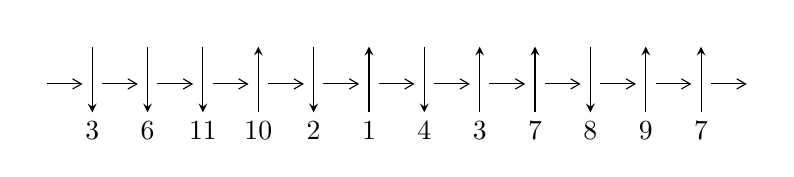
\begin{tikzpicture}[x=20pt, y=17pt]
	% nodes
	\node (C0) at (0, 0) {};
	\node (C1) at (1, 0) {};
	\node (C1U) at (1, +1) {};
	\node (C1D) at (1, -1) {3};

	\node (C2) at (2, 0) {};
	\node (C2U) at (2, +1) {};
	\node (C2D) at (2, -1) {6};

	\node (C3) at (3, 0) {};
	\node (C3U) at (3, +1) {};
	\node (C3D) at (3, -1) {11};

	\node (C4) at (4, 0) {};
	\node (C4U) at (4, +1) {};
	\node (C4D) at (4, -1) {10};

	\node (C5) at (5, 0) {};
	\node (C5U) at (5, +1) {};
	\node (C5D) at (5, -1) {2};

	\node (C6) at (6, 0) {};
	\node (C6U) at (6, +1) {};
	\node (C6D) at (6, -1) {1};

	\node (C7) at (7, 0) {};
	\node (C7U) at (7, +1) {};
	\node (C7D) at (7, -1) {4};

	\node (C8) at (8, 0) {};
	\node (C8U) at (8, +1) {};
	\node (C8D) at (8, -1) {3};

	\node (C9) at (9, 0) {};
	\node (C9U) at (9, +1) {};
	\node (C9D) at (9, -1) {7};

	\node (C10) at (10, 0) {};
	\node (C10U) at (10, +1) {};
	\node (C10D) at (10, -1) {8};

	\node (C11) at (11, 0) {};
	\node (C11U) at (11, +1) {};
	\node (C11D) at (11, -1) {9};

	\node (C12) at (12, 0) {};
	\node (C12U) at (12, +1) {};
	\node (C12D) at (12, -1) {7};
	\node (C13) at (13, 0) {};

	% arrows
	\draw[->,>={angle 60}]
	(C0) edge (C1) (C1) edge (C2) (C2) edge (C3) (C3) edge (C4) (C4) edge (C5) (C5) edge (C6) (C6) edge (C7) (C7) edge (C8) (C8) edge (C9) (C9) edge (C10) (C10) edge (C11) (C11) edge (C12) (C12) edge (C13) ;	\draw[->,>=stealth]
	(C1U) edge (C1D) (C2U) edge (C2D) (C3U) edge (C3D) (C4D) edge (C4U) (C5U) edge (C5D) (C6D) edge (C6U) (C7U) edge (C7D) (C8D) edge (C8U) (C9D) edge (C9U) (C10U) edge (C10D) (C11D) edge (C11U) (C12D) edge (C12U) ;
	\end{tikzpicture} \\
\hhline{~~} \\& 
\textbf{Solving Sequence} \\ \cline{2-2} 
 &
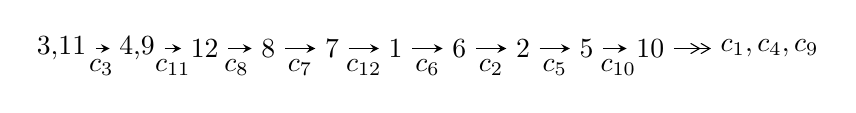
\begin{tikzpicture}[x=23pt, y=7pt]
	% node
	\node (A0) at (-1/8, 0) {3,11};
	\node (A1) at (17/16, 0) {4,9};
	\node (A2) at (17/8, 0) {12};
	\node (A3) at (25/8, 0) {8};
	\node (A4) at (33/8, 0) {7};
	\node (A5) at (41/8, 0) {1};
	\node (A6) at (49/8, 0) {6};
	\node (A7) at (57/8, 0) {2};
	\node (A8) at (65/8, 0) {5};
	\node (A9) at (73/8, 0) {10};
	\node (C1) at (1/2, -1) {$c_{3}$};
	\node (C2) at (13/8, -1) {$c_{11}$};
	\node (C3) at (21/8, -1) {$c_{8}$};
	\node (C4) at (29/8, -1) {$c_{7}$};
	\node (C5) at (37/8, -1) {$c_{12}$};
	\node (C6) at (45/8, -1) {$c_{6}$};
	\node (C7) at (53/8, -1) {$c_{2}$};
	\node (C8) at (61/8, -1) {$c_{5}$};
	\node (C9) at (69/8, -1) {$c_{10}$};
	\node (A10) at (11, 0) {$c_{1},c_{4},c_{9}$};

	% edge
	\draw[->,>=stealth]	
	(A0) edge (A1) (A1) edge (A2) (A2) edge (A3) (A3) edge (A4) (A4) edge (A5) (A5) edge (A6) (A6) edge (A7) (A7) edge (A8) (A8) edge (A9) ;
	\draw[->>,>={angle 60}]	
	(A9) edge (A10);
\end{tikzpicture} \\ 

\end{tabular} \\

\footnotetext{
The image of knot diagram is generated by the software ``\textbf{Draw programme}" developed by Andrew Bartholomew(\url{http://www.layer8.co.uk/maths/draw/index.htm\#Running-draw}), where we modified some parts for our purpose(\url{https://github.com/CATsTAILs/LinksPainter}).
}\phantom \\ \newline 
\centering \textbf{Ideals for irreducible components\footnotemark of $X_{\text{par}}$} 
 
\begin{align*}
I^u_{1}&=\langle 
5.47880\times10^{25} u^{40}+7.88111\times10^{25} u^{39}+\cdots+1.50975\times10^{24} b+6.96929\times10^{25},\\
\phantom{I^u_{1}}&\phantom{= \langle  }-1.08127\times10^{26} u^{40}-1.53797\times10^{26} u^{39}+\cdots+1.50975\times10^{24} a-1.21442\times10^{26},\;u^{41}+u^{40}+\cdots+2 u+1\rangle \\
I^u_{2}&=\langle 
-2.49556\times10^{86} u^{43}-8.35365\times10^{86} u^{42}+\cdots+3.43675\times10^{87} b+3.73757\times10^{87},\\
\phantom{I^u_{2}}&\phantom{= \langle  }2.75946\times10^{87} u^{43}+1.12653\times10^{88} u^{42}+\cdots+5.84247\times10^{88} a+3.07830\times10^{89},\;u^{44}+4 u^{43}+\cdots+77 u+17\rangle \\
I^u_{3}&=\langle 
- u^{18}+u^{17}+\cdots+b+4 u,\;-4 u^{18}+4 u^{17}+\cdots+a-1,\;u^{19}- u^{18}+\cdots-4 u^2+1\rangle \\
I^u_{4}&=\langle 
b- u-1,\;a- u-1,\;u^2+u+1\rangle \\
\\
\end{align*}
\raggedright * 4 irreducible components of $\dim_{\mathbb{C}}=0$, with total 106 representations.\\
\footnotetext{All coefficients of polynomials are rational numbers. But the coefficients are sometimes approximated in decimal forms when there is not enough margin.}
\newpage
\renewcommand{\arraystretch}{1}
\centering \section*{I. $I^u_{1}= \langle 5.48\times10^{25} u^{40}+7.88\times10^{25} u^{39}+\cdots+1.51\times10^{24} b+6.97\times10^{25},\;-1.08\times10^{26} u^{40}-1.54\times10^{26} u^{39}+\cdots+1.51\times10^{24} a-1.21\times10^{26},\;u^{41}+u^{40}+\cdots+2 u+1 \rangle$}
\flushleft \textbf{(i) Arc colorings}\\
\begin{tabular}{m{7pt} m{180pt} m{7pt} m{180pt} }
\flushright $a_{3}=$&$\begin{pmatrix}1\\0\end{pmatrix}$ \\
\flushright $a_{11}=$&$\begin{pmatrix}0\\u\end{pmatrix}$ \\
\flushright $a_{4}=$&$\begin{pmatrix}1\\u^2\end{pmatrix}$ \\
\flushright $a_{9}=$&$\begin{pmatrix}71.6189 u^{40}+101.869 u^{39}+\cdots+340.999 u+80.4384\\-36.2894 u^{40}-52.2014 u^{39}+\cdots-199.232 u-46.1618\end{pmatrix}$ \\
\flushright $a_{12}=$&$\begin{pmatrix}-64.2074 u^{40}-87.5660 u^{39}+\cdots-425.889 u-95.1075\\-18.2487 u^{40}-25.7511 u^{39}+\cdots-53.4475 u-14.3937\end{pmatrix}$ \\
\flushright $a_{8}=$&$\begin{pmatrix}107.908 u^{40}+154.070 u^{39}+\cdots+540.231 u+126.600\\-36.2894 u^{40}-52.2014 u^{39}+\cdots-199.232 u-46.1618\end{pmatrix}$ \\
\flushright $a_{7}=$&$\begin{pmatrix}107.908 u^{40}+154.070 u^{39}+\cdots+541.231 u+126.600\\-36.2894 u^{40}-52.2014 u^{39}+\cdots-199.232 u-46.1618\end{pmatrix}$ \\
\flushright $a_{1}=$&$\begin{pmatrix}-197.492 u^{40}-281.182 u^{39}+\cdots-1214.12 u-264.909\\-0.0153376 u^{40}-1.23868 u^{39}+\cdots+111.193 u+23.1345\end{pmatrix}$ \\
\flushright $a_{6}=$&$\begin{pmatrix}74.2253 u^{40}+243.405 u^{39}+\cdots+1398.14 u+562.092\\39.9044 u^{40}+24.6029 u^{39}+\cdots-18.7145 u-94.6713\end{pmatrix}$ \\
\flushright $a_{2}=$&$\begin{pmatrix}-197.477 u^{40}-279.943 u^{39}+\cdots-1325.31 u-288.043\\-0.0153376 u^{40}-1.23868 u^{39}+\cdots+111.193 u+23.1345\end{pmatrix}$ \\
\flushright $a_{5}=$&$\begin{pmatrix}-64.8577 u^{40}-25.7158 u^{39}+\cdots+90.6679 u+163.055\\-22.8032 u^{40}-1.56551 u^{39}+\cdots+55.9091 u+43.7009\end{pmatrix}$ \\
\flushright $a_{10}=$&$\begin{pmatrix}0.594704 u^{40}+4.62146 u^{39}+\cdots-162.562 u-30.5253\\-46.5535 u^{40}-66.4364 u^{39}+\cdots-207.880 u-50.1886\end{pmatrix}$\\&\end{tabular}
\flushleft \textbf{(ii) Obstruction class $= -1$}\\~\\
\flushleft \textbf{(iii) Cusp Shapes $= \frac{46609776655609602573804741}{1509752124425304287631895} u^{40}-\frac{555844712353330908256438968}{1509752124425304287631895} u^{39}+\cdots-\frac{4270771601823530319752574608}{1509752124425304287631895} u-\frac{2076142798565092784971764701}{1509752124425304287631895}$}\\~\\
\newpage\renewcommand{\arraystretch}{1}
\flushleft \textbf{(iv) u-Polynomials at the component}\newline \\
\begin{tabular}{m{50pt}|m{274pt}}
Crossings & \hspace{64pt}u-Polynomials at each crossing \\
\hline $$\begin{aligned}c_{1}\end{aligned}$$&$\begin{aligned}
&u^{41}+19 u^{40}+\cdots+89 u+16
\end{aligned}$\\
\hline $$\begin{aligned}c_{2},c_{5}\end{aligned}$$&$\begin{aligned}
&u^{41}+5 u^{40}+\cdots+7 u+4
\end{aligned}$\\
\hline $$\begin{aligned}c_{3},c_{7}\end{aligned}$$&$\begin{aligned}
&u^{41}+u^{40}+\cdots+2 u+1
\end{aligned}$\\
\hline $$\begin{aligned}c_{4},c_{8}\end{aligned}$$&$\begin{aligned}
&u^{41}-9 u^{39}+\cdots-69 u+17
\end{aligned}$\\
\hline $$\begin{aligned}c_{6},c_{12}\end{aligned}$$&$\begin{aligned}
&u^{41}+15 u^{40}+\cdots+87 u+4
\end{aligned}$\\
\hline $$\begin{aligned}c_{9},c_{11}\end{aligned}$$&$\begin{aligned}
&u^{41}-4 u^{40}+\cdots+27 u+1
\end{aligned}$\\
\hline $$\begin{aligned}c_{10}\end{aligned}$$&$\begin{aligned}
&u^{41}-26 u^{40}+\cdots+23 u-2
\end{aligned}$\\
\hline
\end{tabular}\\~\\
\newpage\renewcommand{\arraystretch}{1}
\flushleft \textbf{(v) Riley Polynomials at the component}\newline \\
\begin{tabular}{m{50pt}|m{274pt}}
Crossings & \hspace{64pt}Riley Polynomials at each crossing \\
\hline $$\begin{aligned}c_{1}\end{aligned}$$&$\begin{aligned}
&y^{41}+9 y^{40}+\cdots-3311 y-256
\end{aligned}$\\
\hline $$\begin{aligned}c_{2},c_{5}\end{aligned}$$&$\begin{aligned}
&y^{41}-19 y^{40}+\cdots+89 y-16
\end{aligned}$\\
\hline $$\begin{aligned}c_{3},c_{7}\end{aligned}$$&$\begin{aligned}
&y^{41}+17 y^{40}+\cdots-36 y-1
\end{aligned}$\\
\hline $$\begin{aligned}c_{4},c_{8}\end{aligned}$$&$\begin{aligned}
&y^{41}-18 y^{40}+\cdots+5577 y-289
\end{aligned}$\\
\hline $$\begin{aligned}c_{6},c_{12}\end{aligned}$$&$\begin{aligned}
&y^{41}+y^{40}+\cdots+633 y-16
\end{aligned}$\\
\hline $$\begin{aligned}c_{9},c_{11}\end{aligned}$$&$\begin{aligned}
&y^{41}-58 y^{40}+\cdots+333 y-1
\end{aligned}$\\
\hline $$\begin{aligned}c_{10}\end{aligned}$$&$\begin{aligned}
&y^{41}+68 y^{39}+\cdots+81 y-4
\end{aligned}$\\
\hline
\end{tabular}\\~\\
\newpage\flushleft \textbf{(vi) Complex Volumes and Cusp Shapes}
$$\begin{array}{c|c|c}  
\text{Solutions to }I^u_{1}& \I (\text{vol} + \sqrt{-1}CS) & \text{Cusp shape}\\
 \hline 
\begin{aligned}
u &= \phantom{-}0.347021 + 1.021800 I \\
a &= \phantom{-}0.446471 + 0.717252 I \\
b &= \phantom{-}0.856068 + 0.901582 I\end{aligned}
 & \phantom{-}2.01077 + 1.97128 I & \phantom{-0.000000 } 0 \\ \hline\begin{aligned}
u &= \phantom{-}0.347021 - 1.021800 I \\
a &= \phantom{-}0.446471 - 0.717252 I \\
b &= \phantom{-}0.856068 - 0.901582 I\end{aligned}
 & \phantom{-}2.01077 - 1.97128 I & \phantom{-0.000000 } 0 \\ \hline\begin{aligned}
u &= -0.517326 + 0.952123 I \\
a &= -0.494773 + 0.392816 I \\
b &= -1.002680 + 0.556094 I\end{aligned}
 & \phantom{-}2.33608 + 2.70211 I & \phantom{-0.000000 } 0 \\ \hline\begin{aligned}
u &= -0.517326 - 0.952123 I \\
a &= -0.494773 - 0.392816 I \\
b &= -1.002680 - 0.556094 I\end{aligned}
 & \phantom{-}2.33608 - 2.70211 I & \phantom{-0.000000 } 0 \\ \hline\begin{aligned}
u &= -0.380066 + 0.811067 I \\
a &= \phantom{-}0.82614 + 1.79073 I \\
b &= \phantom{-}0.853726 - 0.187521 I\end{aligned}
 & \phantom{-}4.94484 - 5.32421 I & \phantom{-}4.21074 + 0.90918 I \\ \hline\begin{aligned}
u &= -0.380066 - 0.811067 I \\
a &= \phantom{-}0.82614 - 1.79073 I \\
b &= \phantom{-}0.853726 + 0.187521 I\end{aligned}
 & \phantom{-}4.94484 + 5.32421 I & \phantom{-}4.21074 - 0.90918 I \\ \hline\begin{aligned}
u &= \phantom{-}0.054668 + 1.145580 I \\
a &= \phantom{-}0.106091 + 1.208380 I \\
b &= \phantom{-}0.17829 + 1.44060 I\end{aligned}
 & \phantom{-}1.57207 - 1.96637 I & \phantom{-0.000000 } 0 \\ \hline\begin{aligned}
u &= \phantom{-}0.054668 - 1.145580 I \\
a &= \phantom{-}0.106091 - 1.208380 I \\
b &= \phantom{-}0.17829 - 1.44060 I\end{aligned}
 & \phantom{-}1.57207 + 1.96637 I & \phantom{-0.000000 } 0 \\ \hline\begin{aligned}
u &= \phantom{-}0.358415 + 0.770361 I \\
a &= -0.68843 + 2.01808 I \\
b &= -0.906548 - 0.088949 I\end{aligned}
 & \phantom{-}6.85307 + 0.06384 I & \phantom{-}7.45973 + 4.03926 I \\ \hline\begin{aligned}
u &= \phantom{-}0.358415 - 0.770361 I \\
a &= -0.68843 - 2.01808 I \\
b &= -0.906548 + 0.088949 I\end{aligned}
 & \phantom{-}6.85307 - 0.06384 I & \phantom{-}7.45973 - 4.03926 I\\
 \hline 
 \end{array}$$\newpage$$\begin{array}{c|c|c}  
\text{Solutions to }I^u_{1}& \I (\text{vol} + \sqrt{-1}CS) & \text{Cusp shape}\\
 \hline 
\begin{aligned}
u &= -0.045169 + 0.822753 I \\
a &= -0.154528 + 1.094100 I \\
b &= \phantom{-}0.346455 + 0.374027 I\end{aligned}
 & \phantom{-}1.46454 + 1.46331 I & \phantom{-}5.06919 - 4.70044 I \\ \hline\begin{aligned}
u &= -0.045169 - 0.822753 I \\
a &= -0.154528 - 1.094100 I \\
b &= \phantom{-}0.346455 - 0.374027 I\end{aligned}
 & \phantom{-}1.46454 - 1.46331 I & \phantom{-}5.06919 + 4.70044 I \\ \hline\begin{aligned}
u &= -0.229168 + 0.751258 I \\
a &= -0.04740 + 1.82480 I \\
b &= \phantom{-}0.739876 + 0.180844 I\end{aligned}
 & \phantom{-}1.64581 + 1.65716 I & \phantom{-}2.62674 - 4.29220 I \\ \hline\begin{aligned}
u &= -0.229168 - 0.751258 I \\
a &= -0.04740 - 1.82480 I \\
b &= \phantom{-}0.739876 - 0.180844 I\end{aligned}
 & \phantom{-}1.64581 - 1.65716 I & \phantom{-}2.62674 + 4.29220 I \\ \hline\begin{aligned}
u &= \phantom{-}0.325313 + 0.680386 I \\
a &= -0.29563 + 2.60667 I \\
b &= -1.039970 + 0.122963 I\end{aligned}
 & \phantom{-}7.08787 - 2.96529 I & \phantom{-}8.51449 + 5.47804 I \\ \hline\begin{aligned}
u &= \phantom{-}0.325313 - 0.680386 I \\
a &= -0.29563 - 2.60667 I \\
b &= -1.039970 - 0.122963 I\end{aligned}
 & \phantom{-}7.08787 + 2.96529 I & \phantom{-}8.51449 - 5.47804 I \\ \hline\begin{aligned}
u &= -0.314460 + 0.648327 I \\
a &= \phantom{-}0.08581 + 2.85549 I \\
b &= \phantom{-}1.088460 + 0.205257 I\end{aligned}
 & \phantom{-}5.38587 + 8.24752 I & \phantom{-}6.33209 - 10.48383 I \\ \hline\begin{aligned}
u &= -0.314460 - 0.648327 I \\
a &= \phantom{-}0.08581 - 2.85549 I \\
b &= \phantom{-}1.088460 - 0.205257 I\end{aligned}
 & \phantom{-}5.38587 - 8.24752 I & \phantom{-}6.33209 + 10.48383 I \\ \hline\begin{aligned}
u &= \phantom{-}1.054420 + 0.767365 I \\
a &= \phantom{-}0.225727 - 0.075550 I \\
b &= \phantom{-}0.757531 - 0.087155 I\end{aligned}
 & -5.03812 + 0.55979 I & \phantom{-0.000000 } 0 \\ \hline\begin{aligned}
u &= \phantom{-}1.054420 - 0.767365 I \\
a &= \phantom{-}0.225727 + 0.075550 I \\
b &= \phantom{-}0.757531 + 0.087155 I\end{aligned}
 & -5.03812 - 0.55979 I & \phantom{-0.000000 } 0\\
 \hline 
 \end{array}$$\newpage$$\begin{array}{c|c|c}  
\text{Solutions to }I^u_{1}& \I (\text{vol} + \sqrt{-1}CS) & \text{Cusp shape}\\
 \hline 
\begin{aligned}
u &= -0.954640 + 0.895605 I \\
a &= -0.323203 - 0.114281 I \\
b &= -0.907475 - 0.104542 I\end{aligned}
 & -1.12434 + 3.55718 I & \phantom{-0.000000 } 0 \\ \hline\begin{aligned}
u &= -0.954640 - 0.895605 I \\
a &= -0.323203 + 0.114281 I \\
b &= -0.907475 + 0.104542 I\end{aligned}
 & -1.12434 - 3.55718 I & \phantom{-0.000000 } 0 \\ \hline\begin{aligned}
u &= -0.652653\phantom{ +0.000000I} \\
a &= -0.0877425\phantom{ +0.000000I} \\
b &= -0.483905\phantom{ +0.000000I}\end{aligned}
 & -1.46612\phantom{ +0.000000I} & -7.06880\phantom{ +0.000000I} \\ \hline\begin{aligned}
u &= -0.001515 + 0.601854 I \\
a &= -0.852039 + 0.542047 I \\
b &= \phantom{-}0.481262 + 0.639634 I\end{aligned}
 & \phantom{-}0.81408 + 1.37351 I & \phantom{-}2.99559 - 3.76838 I \\ \hline\begin{aligned}
u &= -0.001515 - 0.601854 I \\
a &= -0.852039 - 0.542047 I \\
b &= \phantom{-}0.481262 - 0.639634 I\end{aligned}
 & \phantom{-}0.81408 - 1.37351 I & \phantom{-}2.99559 + 3.76838 I \\ \hline\begin{aligned}
u &= \phantom{-}1.03621 + 0.97465 I \\
a &= \phantom{-}0.272897 - 0.206391 I \\
b &= \phantom{-}0.879946 - 0.246548 I\end{aligned}
 & -4.42034 - 8.30464 I & \phantom{-0.000000 } 0 \\ \hline\begin{aligned}
u &= \phantom{-}1.03621 - 0.97465 I \\
a &= \phantom{-}0.272897 + 0.206391 I \\
b &= \phantom{-}0.879946 + 0.246548 I\end{aligned}
 & -4.42034 + 8.30464 I & \phantom{-0.000000 } 0 \\ \hline\begin{aligned}
u &= \phantom{-}0.051342 + 0.543114 I \\
a &= \phantom{-}1.57833 + 0.32834 I \\
b &= -0.542371 + 0.798966 I\end{aligned}
 & -1.14789 - 5.43637 I & -0.71682 + 6.54388 I \\ \hline\begin{aligned}
u &= \phantom{-}0.051342 - 0.543114 I \\
a &= \phantom{-}1.57833 - 0.32834 I \\
b &= -0.542371 - 0.798966 I\end{aligned}
 & -1.14789 + 5.43637 I & -0.71682 - 6.54388 I \\ \hline\begin{aligned}
u &= -0.005268 + 0.490051 I \\
a &= \phantom{-}0.720841 - 0.530154 I \\
b &= -0.243798 + 0.805884 I\end{aligned}
 & -2.19779 + 1.00862 I & -5.99392 - 1.40222 I\\
 \hline 
 \end{array}$$\newpage$$\begin{array}{c|c|c}  
\text{Solutions to }I^u_{1}& \I (\text{vol} + \sqrt{-1}CS) & \text{Cusp shape}\\
 \hline 
\begin{aligned}
u &= -0.005268 - 0.490051 I \\
a &= \phantom{-}0.720841 + 0.530154 I \\
b &= -0.243798 - 0.805884 I\end{aligned}
 & -2.19779 - 1.00862 I & -5.99392 + 1.40222 I \\ \hline\begin{aligned}
u &= -0.92388 + 1.21329 I \\
a &= -0.693432 - 0.848976 I \\
b &= -1.60443 - 0.79675 I\end{aligned}
 & \phantom{-}7.22406 + 2.19782 I & \phantom{-0.000000 } 0 \\ \hline\begin{aligned}
u &= -0.92388 - 1.21329 I \\
a &= -0.693432 + 0.848976 I \\
b &= -1.60443 + 0.79675 I\end{aligned}
 & \phantom{-}7.22406 - 2.19782 I & \phantom{-0.000000 } 0 \\ \hline\begin{aligned}
u &= \phantom{-}0.93985 + 1.21945 I \\
a &= \phantom{-}0.624751 - 0.961319 I \\
b &= \phantom{-}1.57161 - 0.93510 I\end{aligned}
 & \phantom{-}8.66754 - 7.90114 I & \phantom{-0.000000 } 0 \\ \hline\begin{aligned}
u &= \phantom{-}0.93985 - 1.21945 I \\
a &= \phantom{-}0.624751 + 0.961319 I \\
b &= \phantom{-}1.57161 + 0.93510 I\end{aligned}
 & \phantom{-}8.66754 + 7.90114 I & \phantom{-0.000000 } 0 \\ \hline\begin{aligned}
u &= -0.96302 + 1.20795 I \\
a &= -0.367468 - 0.971278 I \\
b &= -1.31719 - 1.03611 I\end{aligned}
 & \phantom{-}1.99155 + 9.34995 I & \phantom{-0.000000 } 0 \\ \hline\begin{aligned}
u &= -0.96302 - 1.20795 I \\
a &= -0.367468 + 0.971278 I \\
b &= -1.31719 + 1.03611 I\end{aligned}
 & \phantom{-}1.99155 - 9.34995 I & \phantom{-0.000000 } 0 \\ \hline\begin{aligned}
u &= \phantom{-}0.96655 + 1.22224 I \\
a &= \phantom{-}0.421833 - 1.155040 I \\
b &= \phantom{-}1.43574 - 1.19661 I\end{aligned}
 & \phantom{-}7.8645 - 11.8540 I & \phantom{-0.000000 } 0 \\ \hline\begin{aligned}
u &= \phantom{-}0.96655 - 1.22224 I \\
a &= \phantom{-}0.421833 + 1.155040 I \\
b &= \phantom{-}1.43574 + 1.19661 I\end{aligned}
 & \phantom{-}7.8645 + 11.8540 I & \phantom{-0.000000 } 0 \\ \hline\begin{aligned}
u &= -0.97295 + 1.22134 I \\
a &= -0.348119 - 1.207570 I \\
b &= -1.38255 - 1.27245 I\end{aligned}
 & \phantom{-}5.7918 + 17.4569 I & \phantom{-0.000000 } 0\\
 \hline 
 \end{array}$$\newpage$$\begin{array}{c|c|c}  
\text{Solutions to }I^u_{1}& \I (\text{vol} + \sqrt{-1}CS) & \text{Cusp shape}\\
 \hline 
\begin{aligned}
u &= -0.97295 - 1.22134 I \\
a &= -0.348119 + 1.207570 I \\
b &= -1.38255 + 1.27245 I\end{aligned}
 & \phantom{-}5.7918 - 17.4569 I & \phantom{-0.000000 } 0\\
 \hline 
 \end{array}$$\newpage\newpage\renewcommand{\arraystretch}{1}
\centering \section*{II. $I^u_{2}= \langle -2.50\times10^{86} u^{43}-8.35\times10^{86} u^{42}+\cdots+3.44\times10^{87} b+3.74\times10^{87},\;2.76\times10^{87} u^{43}+1.13\times10^{88} u^{42}+\cdots+5.84\times10^{88} a+3.08\times10^{89},\;u^{44}+4 u^{43}+\cdots+77 u+17 \rangle$}
\flushleft \textbf{(i) Arc colorings}\\
\begin{tabular}{m{7pt} m{180pt} m{7pt} m{180pt} }
\flushright $a_{3}=$&$\begin{pmatrix}1\\0\end{pmatrix}$ \\
\flushright $a_{11}=$&$\begin{pmatrix}0\\u\end{pmatrix}$ \\
\flushright $a_{4}=$&$\begin{pmatrix}1\\u^2\end{pmatrix}$ \\
\flushright $a_{9}=$&$\begin{pmatrix}-0.0472311 u^{43}-0.192817 u^{42}+\cdots-14.3118 u-5.26884\\0.0726141 u^{43}+0.243068 u^{42}+\cdots-1.78608 u-1.08753\end{pmatrix}$ \\
\flushright $a_{12}=$&$\begin{pmatrix}-0.0360992 u^{43}-0.157605 u^{42}+\cdots-15.0581 u-5.83261\\0.0702088 u^{43}+0.234463 u^{42}+\cdots-1.55171 u-1.42798\end{pmatrix}$ \\
\flushright $a_{8}=$&$\begin{pmatrix}-0.119845 u^{43}-0.435885 u^{42}+\cdots-12.5257 u-4.18131\\0.0726141 u^{43}+0.243068 u^{42}+\cdots-1.78608 u-1.08753\end{pmatrix}$ \\
\flushright $a_{7}=$&$\begin{pmatrix}-0.0588235 u^{43}-0.235294 u^{42}+\cdots-13 u-4.52941\\0.0610217 u^{43}+0.200591 u^{42}+\cdots+0.525708 u-0.348105\end{pmatrix}$ \\
\flushright $a_{1}=$&$\begin{pmatrix}-0.101101 u^{43}-0.408588 u^{42}+\cdots-18.6194 u-7.52962\\0.00441605 u^{43}-0.0127382 u^{42}+\cdots-3.21768 u-1.61521\end{pmatrix}$ \\
\flushright $a_{6}=$&$\begin{pmatrix}-0.0490639 u^{43}-0.254746 u^{42}+\cdots-9.79483 u-5.26468\\0.0362894 u^{43}+0.127630 u^{42}+\cdots-0.376828 u-1.15074\end{pmatrix}$ \\
\flushright $a_{2}=$&$\begin{pmatrix}-0.105517 u^{43}-0.395849 u^{42}+\cdots-15.4017 u-5.91441\\0.00441605 u^{43}-0.0127382 u^{42}+\cdots-3.21768 u-1.61521\end{pmatrix}$ \\
\flushright $a_{5}=$&$\begin{pmatrix}0.142243 u^{43}+0.513366 u^{42}+\cdots+14.5329 u+3.09094\\-0.00902369 u^{43}-0.0430917 u^{42}+\cdots-3.30811 u-1.10503\end{pmatrix}$ \\
\flushright $a_{10}=$&$\begin{pmatrix}-0.0606353 u^{43}-0.229405 u^{42}+\cdots-7.19891 u-3.39724\\-0.0456727 u^{43}-0.162664 u^{42}+\cdots-4.30750 u-1.00739\end{pmatrix}$\\&\end{tabular}
\flushleft \textbf{(ii) Obstruction class $= -1$}\\~\\
\flushleft \textbf{(iii) Cusp Shapes $= -0.861289 u^{43}-3.44599 u^{42}+\cdots-97.7115 u-26.0425$}\\~\\
\newpage\renewcommand{\arraystretch}{1}
\flushleft \textbf{(iv) u-Polynomials at the component}\newline \\
\begin{tabular}{m{50pt}|m{274pt}}
Crossings & \hspace{64pt}u-Polynomials at each crossing \\
\hline $$\begin{aligned}c_{1}\end{aligned}$$&$\begin{aligned}
&(u^{22}+10 u^{21}+\cdots+6 u^2+1)^{2}
\end{aligned}$\\
\hline $$\begin{aligned}c_{2},c_{5}\end{aligned}$$&$\begin{aligned}
&(u^{22}-2 u^{21}+\cdots-5 u^3+1)^{2}
\end{aligned}$\\
\hline $$\begin{aligned}c_{3},c_{7}\end{aligned}$$&$\begin{aligned}
&u^{44}+4 u^{43}+\cdots+77 u+17
\end{aligned}$\\
\hline $$\begin{aligned}c_{4},c_{8}\end{aligned}$$&$\begin{aligned}
&u^{44}+2 u^{43}+\cdots-7681 u+1663
\end{aligned}$\\
\hline $$\begin{aligned}c_{6},c_{12}\end{aligned}$$&$\begin{aligned}
&(u^{22}-9 u^{21}+\cdots-27 u+8)^{2}
\end{aligned}$\\
\hline $$\begin{aligned}c_{9},c_{11}\end{aligned}$$&$\begin{aligned}
&u^{44}-3 u^{43}+\cdots-5634 u+459
\end{aligned}$\\
\hline $$\begin{aligned}c_{10}\end{aligned}$$&$\begin{aligned}
&(u^{22}+9 u^{21}+\cdots+u+2)^{2}
\end{aligned}$\\
\hline
\end{tabular}\\~\\
\newpage\renewcommand{\arraystretch}{1}
\flushleft \textbf{(v) Riley Polynomials at the component}\newline \\
\begin{tabular}{m{50pt}|m{274pt}}
Crossings & \hspace{64pt}Riley Polynomials at each crossing \\
\hline $$\begin{aligned}c_{1}\end{aligned}$$&$\begin{aligned}
&(y^{22}+6 y^{21}+\cdots+12 y+1)^{2}
\end{aligned}$\\
\hline $$\begin{aligned}c_{2},c_{5}\end{aligned}$$&$\begin{aligned}
&(y^{22}-10 y^{21}+\cdots+6 y^2+1)^{2}
\end{aligned}$\\
\hline $$\begin{aligned}c_{3},c_{7}\end{aligned}$$&$\begin{aligned}
&y^{44}-8 y^{43}+\cdots+1585 y+289
\end{aligned}$\\
\hline $$\begin{aligned}c_{4},c_{8}\end{aligned}$$&$\begin{aligned}
&y^{44}-20 y^{43}+\cdots+60881257 y+2765569
\end{aligned}$\\
\hline $$\begin{aligned}c_{6},c_{12}\end{aligned}$$&$\begin{aligned}
&(y^{22}-5 y^{21}+\cdots-137 y+64)^{2}
\end{aligned}$\\
\hline $$\begin{aligned}c_{9},c_{11}\end{aligned}$$&$\begin{aligned}
&y^{44}-23 y^{43}+\cdots+46259586 y+210681
\end{aligned}$\\
\hline $$\begin{aligned}c_{10}\end{aligned}$$&$\begin{aligned}
&(y^{22}+3 y^{21}+\cdots+43 y+4)^{2}
\end{aligned}$\\
\hline
\end{tabular}\\~\\
\newpage\flushleft \textbf{(vi) Complex Volumes and Cusp Shapes}
$$\begin{array}{c|c|c}  
\text{Solutions to }I^u_{2}& \I (\text{vol} + \sqrt{-1}CS) & \text{Cusp shape}\\
 \hline 
\begin{aligned}
u &= -0.466106 + 0.845310 I \\
a &= \phantom{-}0.120142 + 0.417834 I \\
b &= \phantom{-}1.67800 + 0.61371 I\end{aligned}
 & -0.49172 + 7.76222 I & \phantom{-}0.81633 - 10.97056 I \\ \hline\begin{aligned}
u &= -0.466106 - 0.845310 I \\
a &= \phantom{-}0.120142 - 0.417834 I \\
b &= \phantom{-}1.67800 - 0.61371 I\end{aligned}
 & -0.49172 - 7.76222 I & \phantom{-}0.81633 + 10.97056 I \\ \hline\begin{aligned}
u &= -0.612747 + 0.847167 I \\
a &= -0.309849 + 0.822684 I \\
b &= \phantom{-}1.14999 + 1.06245 I\end{aligned}
 & -2.01009 + 2.56491 I & -5.72976 - 4.00419 I \\ \hline\begin{aligned}
u &= -0.612747 - 0.847167 I \\
a &= -0.309849 - 0.822684 I \\
b &= \phantom{-}1.14999 - 1.06245 I\end{aligned}
 & -2.01009 - 2.56491 I & -5.72976 + 4.00419 I \\ \hline\begin{aligned}
u &= \phantom{-}0.899310 + 0.535213 I \\
a &= \phantom{-}1.22496 + 1.07887 I \\
b &= -0.208918 + 0.720383 I\end{aligned}
 & -2.01009 - 2.56491 I & -5.72976 + 4.00419 I \\ \hline\begin{aligned}
u &= \phantom{-}0.899310 - 0.535213 I \\
a &= \phantom{-}1.22496 - 1.07887 I \\
b &= -0.208918 - 0.720383 I\end{aligned}
 & -2.01009 + 2.56491 I & -5.72976 - 4.00419 I \\ \hline\begin{aligned}
u &= \phantom{-}0.667133 + 0.876190 I \\
a &= \phantom{-}0.565670 + 0.915397 I \\
b &= -0.73275 + 1.28707 I\end{aligned}
 & -2.61181 - 5.56778 I & -6.67774 + 6.14625 I \\ \hline\begin{aligned}
u &= \phantom{-}0.667133 - 0.876190 I \\
a &= \phantom{-}0.565670 - 0.915397 I \\
b &= -0.73275 - 1.28707 I\end{aligned}
 & -2.61181 + 5.56778 I & -6.67774 - 6.14625 I \\ \hline\begin{aligned}
u &= \phantom{-}0.420458 + 0.759517 I \\
a &= \phantom{-}0.0506571 + 0.0690852 I \\
b &= -1.51754 + 0.25724 I\end{aligned}
 & \phantom{-}0.63374 - 3.32247 I & \phantom{-}4.93738 + 4.78079 I \\ \hline\begin{aligned}
u &= \phantom{-}0.420458 - 0.759517 I \\
a &= \phantom{-}0.0506571 - 0.0690852 I \\
b &= -1.51754 - 0.25724 I\end{aligned}
 & \phantom{-}0.63374 + 3.32247 I & \phantom{-}4.93738 - 4.78079 I\\
 \hline 
 \end{array}$$\newpage$$\begin{array}{c|c|c}  
\text{Solutions to }I^u_{2}& \I (\text{vol} + \sqrt{-1}CS) & \text{Cusp shape}\\
 \hline 
\begin{aligned}
u &= \phantom{-}0.592653 + 0.967467 I \\
a &= \phantom{-}0.548691 + 0.593530 I \\
b &= -0.351079 + 1.129330 I\end{aligned}
 & -2.49866 + 0.61650 I & -5.58678 - 1.76375 I \\ \hline\begin{aligned}
u &= \phantom{-}0.592653 - 0.967467 I \\
a &= \phantom{-}0.548691 - 0.593530 I \\
b &= -0.351079 - 1.129330 I\end{aligned}
 & -2.49866 - 0.61650 I & -5.58678 + 1.76375 I \\ \hline\begin{aligned}
u &= -0.510707 + 0.679843 I \\
a &= -0.82932 - 1.56718 I \\
b &= -1.70942 - 1.64533 I\end{aligned}
 & \phantom{-}4.38951 + 8.87036 I & \phantom{-}2.10374 - 11.14588 I \\ \hline\begin{aligned}
u &= -0.510707 - 0.679843 I \\
a &= -0.82932 + 1.56718 I \\
b &= -1.70942 + 1.64533 I\end{aligned}
 & \phantom{-}4.38951 - 8.87036 I & \phantom{-}2.10374 + 11.14588 I \\ \hline\begin{aligned}
u &= -0.748334 + 0.350797 I \\
a &= -1.67537 + 0.57034 I \\
b &= \phantom{-}0.087323 + 0.207716 I\end{aligned}
 & -2.61181 + 5.56778 I & -6.67774 - 6.14625 I \\ \hline\begin{aligned}
u &= -0.748334 - 0.350797 I \\
a &= -1.67537 - 0.57034 I \\
b &= \phantom{-}0.087323 - 0.207716 I\end{aligned}
 & -2.61181 - 5.56778 I & -6.67774 + 6.14625 I \\ \hline\begin{aligned}
u &= \phantom{-}0.438421 + 0.674226 I \\
a &= \phantom{-}0.90058 - 1.59216 I \\
b &= \phantom{-}1.81717 - 1.62217 I\end{aligned}
 & \phantom{-}6.45761 - 3.23482 I & \phantom{-}6.36482 + 6.95069 I \\ \hline\begin{aligned}
u &= \phantom{-}0.438421 - 0.674226 I \\
a &= \phantom{-}0.90058 + 1.59216 I \\
b &= \phantom{-}1.81717 + 1.62217 I\end{aligned}
 & \phantom{-}6.45761 + 3.23482 I & \phantom{-}6.36482 - 6.95069 I \\ \hline\begin{aligned}
u &= -0.784806 + 0.951389 I \\
a &= -0.431263 + 0.864629 I \\
b &= \phantom{-}0.541102 + 0.996237 I\end{aligned}
 & -0.29493 + 2.91734 I & \phantom{-}2.41857 - 2.23849 I \\ \hline\begin{aligned}
u &= -0.784806 - 0.951389 I \\
a &= -0.431263 - 0.864629 I \\
b &= \phantom{-}0.541102 - 0.996237 I\end{aligned}
 & -0.29493 - 2.91734 I & \phantom{-}2.41857 + 2.23849 I\\
 \hline 
 \end{array}$$\newpage$$\begin{array}{c|c|c}  
\text{Solutions to }I^u_{2}& \I (\text{vol} + \sqrt{-1}CS) & \text{Cusp shape}\\
 \hline 
\begin{aligned}
u &= -0.149975 + 0.738011 I \\
a &= -0.89919 - 1.49365 I \\
b &= -2.06203 - 1.36914 I\end{aligned}
 & \phantom{-}5.86334 - 6.33920 I & \phantom{-}7.62789 + 3.75640 I \\ \hline\begin{aligned}
u &= -0.149975 - 0.738011 I \\
a &= -0.89919 + 1.49365 I \\
b &= -2.06203 + 1.36914 I\end{aligned}
 & \phantom{-}5.86334 + 6.33920 I & \phantom{-}7.62789 - 3.75640 I \\ \hline\begin{aligned}
u &= \phantom{-}0.229621 + 0.711467 I \\
a &= \phantom{-}0.93052 - 1.58410 I \\
b &= \phantom{-}2.01034 - 1.49221 I\end{aligned}
 & \phantom{-}7.29150 + 0.70655 I & \phantom{-}9.80660 + 2.74214 I \\ \hline\begin{aligned}
u &= \phantom{-}0.229621 - 0.711467 I \\
a &= \phantom{-}0.93052 + 1.58410 I \\
b &= \phantom{-}2.01034 + 1.49221 I\end{aligned}
 & \phantom{-}7.29150 - 0.70655 I & \phantom{-}9.80660 - 2.74214 I \\ \hline\begin{aligned}
u &= \phantom{-}1.057640 + 0.711303 I \\
a &= \phantom{-}0.72238 + 1.49263 I \\
b &= -0.394766 + 1.085170 I\end{aligned}
 & -0.49172 - 7.76222 I & \phantom{-0.000000 -}0. + 10.97056 I \\ \hline\begin{aligned}
u &= \phantom{-}1.057640 - 0.711303 I \\
a &= \phantom{-}0.72238 - 1.49263 I \\
b &= -0.394766 - 1.085170 I\end{aligned}
 & -0.49172 + 7.76222 I & \phantom{-0.000000 } 0. - 10.97056 I \\ \hline\begin{aligned}
u &= -1.010300 + 0.819633 I \\
a &= -0.496055 + 1.296710 I \\
b &= \phantom{-}0.521329 + 1.021470 I\end{aligned}
 & \phantom{-}0.63374 + 3.32247 I & \phantom{-}4.93738 - 4.78079 I \\ \hline\begin{aligned}
u &= -1.010300 - 0.819633 I \\
a &= -0.496055 - 1.296710 I \\
b &= \phantom{-}0.521329 - 1.021470 I\end{aligned}
 & \phantom{-}0.63374 - 3.32247 I & \phantom{-}4.93738 + 4.78079 I \\ \hline\begin{aligned}
u &= \phantom{-}0.456405 + 0.493869 I \\
a &= \phantom{-}1.008840 - 0.278321 I \\
b &= -0.785235 - 0.137592 I\end{aligned}
 & -0.29493 - 2.91734 I & \phantom{-}2.41857 + 2.23849 I \\ \hline\begin{aligned}
u &= \phantom{-}0.456405 - 0.493869 I \\
a &= \phantom{-}1.008840 + 0.278321 I \\
b &= -0.785235 + 0.137592 I\end{aligned}
 & -0.29493 + 2.91734 I & \phantom{-}2.41857 - 2.23849 I\\
 \hline 
 \end{array}$$\newpage$$\begin{array}{c|c|c}  
\text{Solutions to }I^u_{2}& \I (\text{vol} + \sqrt{-1}CS) & \text{Cusp shape}\\
 \hline 
\begin{aligned}
u &= -0.352482 + 0.507121 I \\
a &= -1.07753 - 1.61193 I \\
b &= -1.91155 - 1.49298 I\end{aligned}
 & \phantom{-}0.543309 + 0.646462 I & \phantom{-}7.41895 - 11.49115 I \\ \hline\begin{aligned}
u &= -0.352482 - 0.507121 I \\
a &= -1.07753 + 1.61193 I \\
b &= -1.91155 + 1.49298 I\end{aligned}
 & \phantom{-}0.543309 - 0.646462 I & \phantom{-}7.41895 + 11.49115 I \\ \hline\begin{aligned}
u &= -0.439360 + 0.215788 I \\
a &= -2.17643 - 0.43074 I \\
b &= \phantom{-}0.249933 - 0.497594 I\end{aligned}
 & -2.49866 - 0.61650 I & -5.58678 + 1.76375 I \\ \hline\begin{aligned}
u &= -0.439360 - 0.215788 I \\
a &= -2.17643 + 0.43074 I \\
b &= \phantom{-}0.249933 + 0.497594 I\end{aligned}
 & -2.49866 + 0.61650 I & -5.58678 - 1.76375 I \\ \hline\begin{aligned}
u &= -1.42727 + 1.17674 I \\
a &= \phantom{-}0.732491 + 0.810544 I \\
b &= \phantom{-}0.999624 + 0.416425 I\end{aligned}
 & \phantom{-}5.86334 + 6.33920 I & \phantom{-0.000000 } 0 \\ \hline\begin{aligned}
u &= -1.42727 - 1.17674 I \\
a &= \phantom{-}0.732491 - 0.810544 I \\
b &= \phantom{-}0.999624 - 0.416425 I\end{aligned}
 & \phantom{-}5.86334 - 6.33920 I & \phantom{-0.000000 } 0 \\ \hline\begin{aligned}
u &= -1.58647 + 1.01845 I \\
a &= \phantom{-}0.919715 + 0.087483 I \\
b &= \phantom{-}0.855383 - 0.305806 I\end{aligned}
 & \phantom{-}4.38951 - 8.87036 I & \phantom{-0.000000 } 0 \\ \hline\begin{aligned}
u &= -1.58647 - 1.01845 I \\
a &= \phantom{-}0.919715 - 0.087483 I \\
b &= \phantom{-}0.855383 + 0.305806 I\end{aligned}
 & \phantom{-}4.38951 + 8.87036 I & \phantom{-0.000000 } 0 \\ \hline\begin{aligned}
u &= \phantom{-}1.49066 + 1.18106 I \\
a &= -0.792313 + 0.634501 I \\
b &= -0.974820 + 0.249567 I\end{aligned}
 & \phantom{-}7.29150 - 0.70655 I & \phantom{-0.000000 } 0 \\ \hline\begin{aligned}
u &= \phantom{-}1.49066 - 1.18106 I \\
a &= -0.792313 - 0.634501 I \\
b &= -0.974820 - 0.249567 I\end{aligned}
 & \phantom{-}7.29150 + 0.70655 I & \phantom{-0.000000 } 0\\
 \hline 
 \end{array}$$\newpage$$\begin{array}{c|c|c}  
\text{Solutions to }I^u_{2}& \I (\text{vol} + \sqrt{-1}CS) & \text{Cusp shape}\\
 \hline 
\begin{aligned}
u &= \phantom{-}1.59443 + 1.07242 I \\
a &= -0.889783 + 0.221269 I \\
b &= -0.883190 - 0.162509 I\end{aligned}
 & \phantom{-}6.45761 + 3.23482 I & \phantom{-0.000000 } 0 \\ \hline\begin{aligned}
u &= \phantom{-}1.59443 - 1.07242 I \\
a &= -0.889783 - 0.221269 I \\
b &= -0.883190 + 0.162509 I\end{aligned}
 & \phantom{-}6.45761 - 3.23482 I & \phantom{-0.000000 } 0 \\ \hline\begin{aligned}
u &= -1.75816 + 1.21062 I \\
a &= \phantom{-}0.587756 + 0.268789 I \\
b &= \phantom{-}0.621112 + 0.027345 I\end{aligned}
 & \phantom{-}0.543309 - 0.646462 I & \phantom{-0.000000 } 0 \\ \hline\begin{aligned}
u &= -1.75816 - 1.21062 I \\
a &= \phantom{-}0.587756 - 0.268789 I \\
b &= \phantom{-}0.621112 - 0.027345 I\end{aligned}
 & \phantom{-}0.543309 + 0.646462 I & \phantom{-0.000000 } 0\\
 \hline 
 \end{array}$$\newpage\newpage\renewcommand{\arraystretch}{1}
\centering \section*{III. $I^u_{3}= \langle - u^{18}+u^{17}+\cdots+b+4 u,\;-4 u^{18}+4 u^{17}+\cdots+a-1,\;u^{19}- u^{18}+\cdots-4 u^2+1 \rangle$}
\flushleft \textbf{(i) Arc colorings}\\
\begin{tabular}{m{7pt} m{180pt} m{7pt} m{180pt} }
\flushright $a_{3}=$&$\begin{pmatrix}1\\0\end{pmatrix}$ \\
\flushright $a_{11}=$&$\begin{pmatrix}0\\u\end{pmatrix}$ \\
\flushright $a_{4}=$&$\begin{pmatrix}1\\u^2\end{pmatrix}$ \\
\flushright $a_{9}=$&$\begin{pmatrix}4 u^{18}-4 u^{17}+\cdots-8 u+1\\u^{18}- u^{17}+\cdots+u^2-4 u\end{pmatrix}$ \\
\flushright $a_{12}=$&$\begin{pmatrix}-8 u^{18}+9 u^{17}+\cdots+14 u-4\\-4 u^{18}+4 u^{17}+\cdots+9 u-1\end{pmatrix}$ \\
\flushright $a_{8}=$&$\begin{pmatrix}3 u^{18}-3 u^{17}+\cdots-4 u+1\\u^{18}- u^{17}+\cdots+u^2-4 u\end{pmatrix}$ \\
\flushright $a_{7}=$&$\begin{pmatrix}3 u^{18}-3 u^{17}+\cdots-5 u+1\\u^{18}- u^{17}+\cdots+u^2-4 u\end{pmatrix}$ \\
\flushright $a_{1}=$&$\begin{pmatrix}- u^{18}+2 u^{16}+\cdots+5 u^2-2\\2 u^{18}-3 u^{17}+\cdots-3 u+2\end{pmatrix}$ \\
\flushright $a_{6}=$&$\begin{pmatrix}-4 u^{18}+5 u^{17}+\cdots-6 u^2+8 u\\3 u^{18}-3 u^{17}+\cdots+9 u^3-3 u\end{pmatrix}$ \\
\flushright $a_{2}=$&$\begin{pmatrix}-3 u^{18}+3 u^{17}+\cdots+3 u-4\\2 u^{18}-3 u^{17}+\cdots-3 u+2\end{pmatrix}$ \\
\flushright $a_{5}=$&$\begin{pmatrix}-2 u^{18}+3 u^{17}+\cdots-3 u^3-1\\- u^{18}+4 u^{17}+\cdots+3 u-5\end{pmatrix}$ \\
\flushright $a_{10}=$&$\begin{pmatrix}- u^{18}+2 u^{17}+\cdots+2 u-2\\-3 u^{18}+3 u^{17}+\cdots+5 u-1\end{pmatrix}$\\&\end{tabular}
\flushleft \textbf{(ii) Obstruction class $= 1$}\\~\\
\flushleft \textbf{(iii) Cusp Shapes $= -7 u^{18}+12 u^{17}+u^{16}-22 u^{15}-16 u^{14}+59 u^{13}-18 u^{12}-76 u^{11}+20 u^{10}+87 u^9-54 u^8-93 u^7+68 u^6+56 u^5-50 u^4-29 u^3+45 u^2+11 u-15$}\\~\\
\newpage\renewcommand{\arraystretch}{1}
\flushleft \textbf{(iv) u-Polynomials at the component}\newline \\
\begin{tabular}{m{50pt}|m{274pt}}
Crossings & \hspace{64pt}u-Polynomials at each crossing \\
\hline $$\begin{aligned}c_{1}\end{aligned}$$&$\begin{aligned}
&u^{19}-10 u^{18}+\cdots+4 u-1
\end{aligned}$\\
\hline $$\begin{aligned}c_{2}\end{aligned}$$&$\begin{aligned}
&u^{19}+2 u^{18}+\cdots-2 u-1
\end{aligned}$\\
\hline $$\begin{aligned}c_{3},c_{7}\end{aligned}$$&$\begin{aligned}
&u^{19}- u^{18}+\cdots-4 u^2+1
\end{aligned}$\\
\hline $$\begin{aligned}c_{4},c_{8}\end{aligned}$$&$\begin{aligned}
&u^{19}-4 u^{17}+\cdots- u+1
\end{aligned}$\\
\hline $$\begin{aligned}c_{5}\end{aligned}$$&$\begin{aligned}
&u^{19}-2 u^{18}+\cdots-2 u+1
\end{aligned}$\\
\hline $$\begin{aligned}c_{6}\end{aligned}$$&$\begin{aligned}
&u^{19}-6 u^{18}+\cdots+14 u-3
\end{aligned}$\\
\hline $$\begin{aligned}c_{9},c_{11}\end{aligned}$$&$\begin{aligned}
&u^{19}-8 u^{18}+\cdots+5 u-1
\end{aligned}$\\
\hline $$\begin{aligned}c_{10}\end{aligned}$$&$\begin{aligned}
&u^{19}+11 u^{18}+\cdots+u-3
\end{aligned}$\\
\hline $$\begin{aligned}c_{12}\end{aligned}$$&$\begin{aligned}
&u^{19}+6 u^{18}+\cdots+14 u+3
\end{aligned}$\\
\hline
\end{tabular}\\~\\
\newpage\renewcommand{\arraystretch}{1}
\flushleft \textbf{(v) Riley Polynomials at the component}\newline \\
\begin{tabular}{m{50pt}|m{274pt}}
Crossings & \hspace{64pt}Riley Polynomials at each crossing \\
\hline $$\begin{aligned}c_{1}\end{aligned}$$&$\begin{aligned}
&y^{19}+2 y^{18}+\cdots+74 y^3-1
\end{aligned}$\\
\hline $$\begin{aligned}c_{2},c_{5}\end{aligned}$$&$\begin{aligned}
&y^{19}-10 y^{18}+\cdots+4 y-1
\end{aligned}$\\
\hline $$\begin{aligned}c_{3},c_{7}\end{aligned}$$&$\begin{aligned}
&y^{19}-5 y^{18}+\cdots+8 y-1
\end{aligned}$\\
\hline $$\begin{aligned}c_{4},c_{8}\end{aligned}$$&$\begin{aligned}
&y^{19}-8 y^{18}+\cdots+5 y-1
\end{aligned}$\\
\hline $$\begin{aligned}c_{6},c_{12}\end{aligned}$$&$\begin{aligned}
&y^{19}+6 y^{18}+\cdots+88 y-9
\end{aligned}$\\
\hline $$\begin{aligned}c_{9},c_{11}\end{aligned}$$&$\begin{aligned}
&y^{19}-16 y^{17}+\cdots-19 y-1
\end{aligned}$\\
\hline $$\begin{aligned}c_{10}\end{aligned}$$&$\begin{aligned}
&y^{19}-3 y^{18}+\cdots+217 y-9
\end{aligned}$\\
\hline
\end{tabular}\\~\\
\newpage\flushleft \textbf{(vi) Complex Volumes and Cusp Shapes}
$$\begin{array}{c|c|c}  
\text{Solutions to }I^u_{3}& \I (\text{vol} + \sqrt{-1}CS) & \text{Cusp shape}\\
 \hline 
\begin{aligned}
u &= \phantom{-}0.571670 + 0.772339 I \\
a &= \phantom{-}1.062330 + 0.376696 I \\
b &= -0.619150 + 0.836486 I\end{aligned}
 & -1.93329 - 0.79135 I & -1.90450 + 1.96423 I \\ \hline\begin{aligned}
u &= \phantom{-}0.571670 - 0.772339 I \\
a &= \phantom{-}1.062330 - 0.376696 I \\
b &= -0.619150 - 0.836486 I\end{aligned}
 & -1.93329 + 0.79135 I & -1.90450 - 1.96423 I \\ \hline\begin{aligned}
u &= -0.691700 + 0.817412 I \\
a &= -0.700220 + 0.415999 I \\
b &= \phantom{-}0.603256 + 0.712894 I\end{aligned}
 & -0.67906 + 4.36107 I & \phantom{-}0.50991 - 7.74806 I \\ \hline\begin{aligned}
u &= -0.691700 - 0.817412 I \\
a &= -0.700220 - 0.415999 I \\
b &= \phantom{-}0.603256 - 0.712894 I\end{aligned}
 & -0.67906 - 4.36107 I & \phantom{-}0.50991 + 7.74806 I \\ \hline\begin{aligned}
u &= -0.694686 + 0.594925 I \\
a &= -0.687377 + 1.111670 I \\
b &= \phantom{-}0.830443 + 0.711186 I\end{aligned}
 & -0.66120 + 2.86463 I & -0.58084 - 3.68051 I \\ \hline\begin{aligned}
u &= -0.694686 - 0.594925 I \\
a &= -0.687377 - 1.111670 I \\
b &= \phantom{-}0.830443 - 0.711186 I\end{aligned}
 & -0.66120 - 2.86463 I & -0.58084 + 3.68051 I \\ \hline\begin{aligned}
u &= -0.901419\phantom{ +0.000000I} \\
a &= \phantom{-}1.36528\phantom{ +0.000000I} \\
b &= \phantom{-}1.10936\phantom{ +0.000000I}\end{aligned}
 & \phantom{-}0.308220\phantom{ +0.000000I} & -0.909270\phantom{ +0.000000I} \\ \hline\begin{aligned}
u &= \phantom{-}0.590402 + 0.625214 I \\
a &= \phantom{-}1.20330 + 1.01252 I \\
b &= -0.798416 + 0.845493 I\end{aligned}
 & -1.76829 - 6.62156 I & -2.87860 + 10.87292 I \\ \hline\begin{aligned}
u &= \phantom{-}0.590402 - 0.625214 I \\
a &= \phantom{-}1.20330 - 1.01252 I \\
b &= -0.798416 - 0.845493 I\end{aligned}
 & -1.76829 + 6.62156 I & -2.87860 - 10.87292 I \\ \hline\begin{aligned}
u &= \phantom{-}0.769919 + 0.066620 I \\
a &= -2.09450 + 0.55481 I \\
b &= -1.289190 + 0.111552 I\end{aligned}
 & \phantom{-}6.31789 - 1.80381 I & \phantom{-}3.64499 + 0.37370 I\\
 \hline 
 \end{array}$$\newpage$$\begin{array}{c|c|c}  
\text{Solutions to }I^u_{3}& \I (\text{vol} + \sqrt{-1}CS) & \text{Cusp shape}\\
 \hline 
\begin{aligned}
u &= \phantom{-}0.769919 - 0.066620 I \\
a &= -2.09450 - 0.55481 I \\
b &= -1.289190 - 0.111552 I\end{aligned}
 & \phantom{-}6.31789 + 1.80381 I & \phantom{-}3.64499 - 0.37370 I \\ \hline\begin{aligned}
u &= -0.756714 + 0.118401 I \\
a &= \phantom{-}1.98867 + 0.99926 I \\
b &= \phantom{-}1.289920 + 0.201830 I\end{aligned}
 & \phantom{-}4.58239 + 7.30195 I & \phantom{-}0.96040 - 5.11591 I \\ \hline\begin{aligned}
u &= -0.756714 - 0.118401 I \\
a &= \phantom{-}1.98867 - 0.99926 I \\
b &= \phantom{-}1.289920 - 0.201830 I\end{aligned}
 & \phantom{-}4.58239 - 7.30195 I & \phantom{-}0.96040 + 5.11591 I \\ \hline\begin{aligned}
u &= -0.966965 + 0.774347 I \\
a &= -0.231110 + 0.472518 I \\
b &= \phantom{-}0.630095 + 0.504581 I\end{aligned}
 & -2.00054 + 3.89777 I & -3.98253 - 5.34580 I \\ \hline\begin{aligned}
u &= -0.966965 - 0.774347 I \\
a &= -0.231110 - 0.472518 I \\
b &= \phantom{-}0.630095 - 0.504581 I\end{aligned}
 & -2.00054 - 3.89777 I & -3.98253 + 5.34580 I \\ \hline\begin{aligned}
u &= \phantom{-}1.100580 + 0.706359 I \\
a &= \phantom{-}0.062826 + 0.442679 I \\
b &= -0.643531 + 0.413021 I\end{aligned}
 & -5.47313 + 0.16274 I & -9.10286 + 4.27042 I \\ \hline\begin{aligned}
u &= \phantom{-}1.100580 - 0.706359 I \\
a &= \phantom{-}0.062826 - 0.442679 I \\
b &= -0.643531 - 0.413021 I\end{aligned}
 & -5.47313 - 0.16274 I & -9.10286 - 4.27042 I \\ \hline\begin{aligned}
u &= \phantom{-}1.028200 + 0.886045 I \\
a &= \phantom{-}0.213453 + 0.338188 I \\
b &= -0.558115 + 0.480952 I\end{aligned}
 & -5.11861 - 8.27352 I & -8.71133 + 6.81608 I \\ \hline\begin{aligned}
u &= \phantom{-}1.028200 - 0.886045 I \\
a &= \phantom{-}0.213453 - 0.338188 I \\
b &= -0.558115 - 0.480952 I\end{aligned}
 & -5.11861 + 8.27352 I & -8.71133 - 6.81608 I\\
 \hline 
 \end{array}$$\newpage\newpage\renewcommand{\arraystretch}{1}
\centering \section*{IV. $I^u_{4}= \langle b- u-1,\;a- u-1,\;u^2+u+1 \rangle$}
\flushleft \textbf{(i) Arc colorings}\\
\begin{tabular}{m{7pt} m{180pt} m{7pt} m{180pt} }
\flushright $a_{3}=$&$\begin{pmatrix}1\\0\end{pmatrix}$ \\
\flushright $a_{11}=$&$\begin{pmatrix}0\\u\end{pmatrix}$ \\
\flushright $a_{4}=$&$\begin{pmatrix}1\\- u-1\end{pmatrix}$ \\
\flushright $a_{9}=$&$\begin{pmatrix}u+1\\u+1\end{pmatrix}$ \\
\flushright $a_{12}=$&$\begin{pmatrix}- u-1\\-1\end{pmatrix}$ \\
\flushright $a_{8}=$&$\begin{pmatrix}0\\u+1\end{pmatrix}$ \\
\flushright $a_{7}=$&$\begin{pmatrix}u+1\\1\end{pmatrix}$ \\
\flushright $a_{1}=$&$\begin{pmatrix}- u-1\\-1\end{pmatrix}$ \\
\flushright $a_{6}=$&$\begin{pmatrix}u+1\\1\end{pmatrix}$ \\
\flushright $a_{2}=$&$\begin{pmatrix}- u\\-1\end{pmatrix}$ \\
\flushright $a_{5}=$&$\begin{pmatrix}1\\0\end{pmatrix}$ \\
\flushright $a_{10}=$&$\begin{pmatrix}0\\u\end{pmatrix}$\\&\end{tabular}
\flushleft \textbf{(ii) Obstruction class $= 1$}\\~\\
\flushleft \textbf{(iii) Cusp Shapes $= -3$}\\~\\
\newpage\renewcommand{\arraystretch}{1}
\flushleft \textbf{(iv) u-Polynomials at the component}\newline \\
\begin{tabular}{m{50pt}|m{274pt}}
Crossings & \hspace{64pt}u-Polynomials at each crossing \\
\hline $$\begin{aligned}c_{1},c_{2},c_{9}\\c_{11}\end{aligned}$$&$\begin{aligned}
&(u-1)^2
\end{aligned}$\\
\hline $$\begin{aligned}c_{3},c_{4},c_{7}\\c_{8}\end{aligned}$$&$\begin{aligned}
&u^2+u+1
\end{aligned}$\\
\hline $$\begin{aligned}c_{5}\end{aligned}$$&$\begin{aligned}
&(u+1)^2
\end{aligned}$\\
\hline $$\begin{aligned}c_{6},c_{10},c_{12}\end{aligned}$$&$\begin{aligned}
&u^2
\end{aligned}$\\
\hline
\end{tabular}\\~\\
\newpage\renewcommand{\arraystretch}{1}
\flushleft \textbf{(v) Riley Polynomials at the component}\newline \\
\begin{tabular}{m{50pt}|m{274pt}}
Crossings & \hspace{64pt}Riley Polynomials at each crossing \\
\hline $$\begin{aligned}c_{1},c_{2},c_{5}\\c_{9},c_{11}\end{aligned}$$&$\begin{aligned}
&(y-1)^2
\end{aligned}$\\
\hline $$\begin{aligned}c_{3},c_{4},c_{7}\\c_{8}\end{aligned}$$&$\begin{aligned}
&y^2+y+1
\end{aligned}$\\
\hline $$\begin{aligned}c_{6},c_{10},c_{12}\end{aligned}$$&$\begin{aligned}
&y^2
\end{aligned}$\\
\hline
\end{tabular}\\~\\
\newpage\flushleft \textbf{(vi) Complex Volumes and Cusp Shapes}
$$\begin{array}{c|c|c}  
\text{Solutions to }I^u_{4}& \I (\text{vol} + \sqrt{-1}CS) & \text{Cusp shape}\\
 \hline 
\begin{aligned}
u &= -0.500000 + 0.866025 I \\
a &= \phantom{-}0.500000 + 0.866025 I \\
b &= \phantom{-}0.500000 + 0.866025 I\end{aligned}
 & \phantom{-0.000000 } 0 & -3.00000\phantom{ +0.000000I} \\ \hline\begin{aligned}
u &= -0.500000 - 0.866025 I \\
a &= \phantom{-}0.500000 - 0.866025 I \\
b &= \phantom{-}0.500000 - 0.866025 I\end{aligned}
 & \phantom{-0.000000 } 0 & -3.00000\phantom{ +0.000000I}\\
 \hline 
 \end{array}$$\newpage
\newpage\renewcommand{\arraystretch}{1}
\centering \section*{ V. u-Polynomials}
\begin{tabular}{m{50pt}|m{274pt}}
Crossings & \hspace{64pt}u-Polynomials at each crossing \\
\hline $$\begin{aligned}c_{1}\end{aligned}$$&$\begin{aligned}
&((u-1)^2)(u^{19}-10 u^{18}+\cdots+4 u-1)(u^{22}+10 u^{21}+\cdots+6 u^2+1)^{2}\\
&\cdot(u^{41}+19 u^{40}+\cdots+89 u+16)
\end{aligned}$\\
\hline $$\begin{aligned}c_{2}\end{aligned}$$&$\begin{aligned}
&((u-1)^2)(u^{19}+2 u^{18}+\cdots-2 u-1)(u^{22}-2 u^{21}+\cdots-5 u^3+1)^{2}\\
&\cdot(u^{41}+5 u^{40}+\cdots+7 u+4)
\end{aligned}$\\
\hline $$\begin{aligned}c_{3},c_{7}\end{aligned}$$&$\begin{aligned}
&(u^2+u+1)(u^{19}- u^{18}+\cdots-4 u^2+1)(u^{41}+u^{40}+\cdots+2 u+1)\\
&\cdot(u^{44}+4 u^{43}+\cdots+77 u+17)
\end{aligned}$\\
\hline $$\begin{aligned}c_{4},c_{8}\end{aligned}$$&$\begin{aligned}
&(u^2+u+1)(u^{19}-4 u^{17}+\cdots- u+1)(u^{41}-9 u^{39}+\cdots-69 u+17)\\
&\cdot(u^{44}+2 u^{43}+\cdots-7681 u+1663)
\end{aligned}$\\
\hline $$\begin{aligned}c_{5}\end{aligned}$$&$\begin{aligned}
&((u+1)^2)(u^{19}-2 u^{18}+\cdots-2 u+1)(u^{22}-2 u^{21}+\cdots-5 u^3+1)^{2}\\
&\cdot(u^{41}+5 u^{40}+\cdots+7 u+4)
\end{aligned}$\\
\hline $$\begin{aligned}c_{6}\end{aligned}$$&$\begin{aligned}
&u^2(u^{19}-6 u^{18}+\cdots+14 u-3)(u^{22}-9 u^{21}+\cdots-27 u+8)^{2}\\
&\cdot(u^{41}+15 u^{40}+\cdots+87 u+4)
\end{aligned}$\\
\hline $$\begin{aligned}c_{9},c_{11}\end{aligned}$$&$\begin{aligned}
&((u-1)^2)(u^{19}-8 u^{18}+\cdots+5 u-1)(u^{41}-4 u^{40}+\cdots+27 u+1)\\
&\cdot(u^{44}-3 u^{43}+\cdots-5634 u+459)
\end{aligned}$\\
\hline $$\begin{aligned}c_{10}\end{aligned}$$&$\begin{aligned}
&u^2(u^{19}+11 u^{18}+\cdots+u-3)(u^{22}+9 u^{21}+\cdots+u+2)^{2}\\
&\cdot(u^{41}-26 u^{40}+\cdots+23 u-2)
\end{aligned}$\\
\hline $$\begin{aligned}c_{12}\end{aligned}$$&$\begin{aligned}
&u^2(u^{19}+6 u^{18}+\cdots+14 u+3)(u^{22}-9 u^{21}+\cdots-27 u+8)^{2}\\
&\cdot(u^{41}+15 u^{40}+\cdots+87 u+4)
\end{aligned}$\\
\hline
\end{tabular}\newpage\renewcommand{\arraystretch}{1}
\centering \section*{ VI. Riley Polynomials}
\begin{tabular}{m{50pt}|m{274pt}}
Crossings & \hspace{64pt}Riley Polynomials at each crossing \\
\hline $$\begin{aligned}c_{1}\end{aligned}$$&$\begin{aligned}
&((y-1)^2)(y^{19}+2 y^{18}+\cdots+74 y^3-1)(y^{22}+6 y^{21}+\cdots+12 y+1)^{2}\\
&\cdot(y^{41}+9 y^{40}+\cdots-3311 y-256)
\end{aligned}$\\
\hline $$\begin{aligned}c_{2},c_{5}\end{aligned}$$&$\begin{aligned}
&((y-1)^2)(y^{19}-10 y^{18}+\cdots+4 y-1)(y^{22}-10 y^{21}+\cdots+6 y^2+1)^{2}\\
&\cdot(y^{41}-19 y^{40}+\cdots+89 y-16)
\end{aligned}$\\
\hline $$\begin{aligned}c_{3},c_{7}\end{aligned}$$&$\begin{aligned}
&(y^2+y+1)(y^{19}-5 y^{18}+\cdots+8 y-1)(y^{41}+17 y^{40}+\cdots-36 y-1)\\
&\cdot(y^{44}-8 y^{43}+\cdots+1585 y+289)
\end{aligned}$\\
\hline $$\begin{aligned}c_{4},c_{8}\end{aligned}$$&$\begin{aligned}
&(y^2+y+1)(y^{19}-8 y^{18}+\cdots+5 y-1)(y^{41}-18 y^{40}+\cdots+5577 y-289)\\
&\cdot(y^{44}-20 y^{43}+\cdots+60881257 y+2765569)
\end{aligned}$\\
\hline $$\begin{aligned}c_{6},c_{12}\end{aligned}$$&$\begin{aligned}
&y^2(y^{19}+6 y^{18}+\cdots+88 y-9)(y^{22}-5 y^{21}+\cdots-137 y+64)^{2}\\
&\cdot(y^{41}+y^{40}+\cdots+633 y-16)
\end{aligned}$\\
\hline $$\begin{aligned}c_{9},c_{11}\end{aligned}$$&$\begin{aligned}
&((y-1)^2)(y^{19}-16 y^{17}+\cdots-19 y-1)(y^{41}-58 y^{40}+\cdots+333 y-1)\\
&\cdot(y^{44}-23 y^{43}+\cdots+46259586 y+210681)
\end{aligned}$\\
\hline $$\begin{aligned}c_{10}\end{aligned}$$&$\begin{aligned}
&y^2(y^{19}-3 y^{18}+\cdots+217 y-9)(y^{22}+3 y^{21}+\cdots+43 y+4)^{2}\\
&\cdot(y^{41}+68 y^{39}+\cdots+81 y-4)
\end{aligned}$\\
\hline
\end{tabular}
\vskip 2pc
\end{document}